\documentclass[a4paper,12pt]{article}
% Package to make citations superscrit with brackets
\usepackage[super,square]{natbib}
% Package to change margin size
\usepackage{anysize}
\usepackage{amsmath}
\marginsize{2cm}{2cm}{1cm}{2cm}
% Package to make headers
\usepackage{fancyhdr}
\usepackage{circuitikz}
\renewcommand{\headrulewidth}{0pt}
\usepackage{soul}
\usepackage[section]{placeins}
% Colors for the references links
\usepackage[dvipsnames]{xcolor}
% Package to link references
\usepackage{hyperref}
\usepackage{graphicx}
\hypersetup{
    colorlinks=true,
    linkcolor=black,
    citecolor=CadetBlue,
    filecolor=CadetBlue,      
    urlcolor=CadetBlue,
}
% Package for lorem ipsum
\usepackage{lipsum}
% Package for multicolumn
\usepackage{multicol}
% Package for removing paragraph identations
\usepackage{parskip}
\setlength\columnsep{18pt}
% Sets bastract
\renewenvironment{abstract}
 {\par\noindent\textbf{\abstractname}\ \ignorespaces \\}
 {\par\noindent\medskip}



 
\begin{document}
% Makes header
\pagestyle{fancy}
\thispagestyle{empty}
\fancyhead[R]{\textit{EE1200}}
\fancyhead[L]{}
% Makes footnotes with an asterisk
\renewcommand*{\thefootnote}{\fnsymbol{footnote}}
\begin{center}
\Large{\textbf{Experiment 04}}
\vspace{0.4cm}
\normalsize
\\ Aditya Tripathy - ee24btech11001, Durgi Swaraj Sharma - ee24btech11018\\
\medskip
\normalsize
\end{center}
{\color{gray}\hrule}
\vspace{0.4cm}
\begin{abstract}
In Experiment-04, we try to capture LC oscillations.
\end{abstract}
{\color{gray}\hrule}
\medskip
\section{Objective}
To study the response of a series RLC circuit with a precharged capacitor.

\section{Apparatus}
\begin{itemize}
\item Oscilloscope
\item Regulated DC power supply
\item Connecting wires and probes
\item Unpolarised capacitor (560$pF$)
\item Inductor (2.2$mH$)
\item Switch (Button switch)
\end{itemize}
\section{Theory}
\begin{figure}[!ht]
\centering
\resizebox{0.5\textwidth}{!}{%
\begin{circuitikz}
  \draw (6,14.5) to[R] (8,14.5);
\draw (8,14.5) to[L ] (9.25,14.5);
\draw (9.25,14.5) to[C] (12,14.5);
\draw (6,14.5) to[short] (5,14.5);
\draw (5,14.5) to[short] (5,12.25);
\draw (5,12.25) to[short] (12,12.25);
\node [font=\normalsize] at (11,17.5) {5V};
\draw (9.25,16.75) to[opening switch,l={ \normalsize t=0}] (10.5,16.75);
\draw (12,14.5) to[closing switch] (12,12.25);
\draw (10.5,16.75) to[american voltage source] (11.75,16.75);
\draw (12,14.5) to[short] (12,16.75);
\draw (9.25,16.75) to[short] (9.25,14.5);
\draw (11.5,16.75) to[short] (12,16.75);
\node [font=\normalsize] at (12.75,13.25) {t=0};
\end{circuitikz}
}%
\label{fig:my_label}
\end{figure}
The resposnse to the circuit shown is the solution to the initial value problem:
\begin{align}
  L\frac{di}{dt} + iR + \frac{q}{C} = 0
\end{align}
with $q(0) = CV_0$ and $i(0) = 0$
\newline
\newline
Since,
\begin{align}
  q = CV_c\\
  \rightarrow i = C\frac{dV_c}{dt}
\end{align}
Now the equation becomes,
\begin{align}
  LC\frac{d^2V_c}{dt^2} + RC\frac{dV_c}{dt} + V_c = 0 
\end{align}
with $V_c(0) = V_0$ and ${V_c}^{\prime}(0) = 0$ 
\newline
The complementary solution to the differential equation is given by 
\begin{align}
  y_c = c_1e^{s_1t} + ce^{s_2t}
\end{align}
where $s_1, s_2$ are solutions to the following quadratic equation
\begin{align}
  LCs^2 + RCs + 1 = 0
\end{align}
Therefore,
\begin{align}
  s_1, s_2 = -\frac{R}{2L} \pm \sqrt{\left(\frac{R}{2L}\right)^2 - \frac{1}{LC}}
\end{align}
Since we wish to study the underdamped case for RLC response, 
\begin{align}
  \left( \frac{R}{2L} \right)^2  - \frac{1}{LC} < 0
\end{align}
Now the complementary solution can be written more conveniently as
\begin{align}
  y_c = e^{-\beta}(c_1 \cos(w_d t) + c_2 \sin(w_d t))
\end{align}
where
\begin{align}
  \beta &= \text{Damping Factor} = \frac{R}{2L}\\
  w_n &= \text{Natural Frequency} = \frac{1}{\sqrt{LC}}\\
  w_d &= \text{Damped Resonance Frequency} = \sqrt{{w_n}^2 - \beta ^ 2}
\end{align}
Now plugging in the initial conditions we get,
\begin{align}
  c_1 = V_0\\
  c_2 = \frac{RV_0}{2Lw_d}
\end{align}
Therefore 
\begin{align}
  V_c(t) = V_0e^{-\beta t}(\cos(w_d t) + \left(\frac{R}{2Lw_d}\right)\sin(w_d t))
\end{align}
\section{Procedure}
\begin{enumerate}
\item Connections
\begin{itemize}
\item Connect the inductor and capacitor in series.
\item Connect the 5V DC Voltage source in parallel to the capacitor.
\item Complete the circuit by adding a switch.
\item Connect the probe across the inductor to capture the voltage response.
\end{itemize}
\item Device Setup
\begin{itemize}
\item To capture the response for the first few cycles, set an appropriate trigger level, set "Sweep = Normal" under "Mode Coupling" and press the "Single" button on the oscilloscope.
\end{itemize}
\item To capture the RLC oscillations, remove the wires connecting DC power supply to capacitor and press the button switch.
\end{enumerate}
\section{Readings}
\begin{table}[htbp]
  \centering\begin{tabular}{|c|c|c|}
    \hline
    Peak No. & Voltage Value & Time Difference($\mu s$)\\
    \hline
    1. & 3.6 & 0 \\
    \hline
    2. & 3.2 & 2.96 \\
    \hline
    3. & 3.0 & 5.92 \\
    \hline
    4. & 2.8 & 8.88 \\
    \hline
    5. & 2.6 & 11.92 \\
    \hline
    6. & 2.2 & 17.84 \\
    \hline
  \end{tabular}
\end{table}
It should be noted that the time difference is measured with respect to first peak.
\section{Results}
Experimental value of $w_d$ = $\frac{2\pi}{2.96 \mu s}$ = 2122697.738912022 $rad/s$\\
Experimental value of $\beta$ = $\frac{\frac{1}{\Delta T_2}\ln{\frac{V_1}{V_2}}  
+ \frac{1}{\Delta T_3}\ln{\frac{V_1}{V_3}}+ \frac{1}{\Delta T_4}\ln{\frac{V_1}{V_4}}+ \frac{1}{\Delta T_5}\ln{\frac{V_1}{V_5}}+ \frac{1}{\Delta T_6}\ln{\frac{V_1}{V_6}}}{5}$ = 30759.2043
$\Omega / H$\\

\section{Response captured}
\begin{figure}[!htb]
  {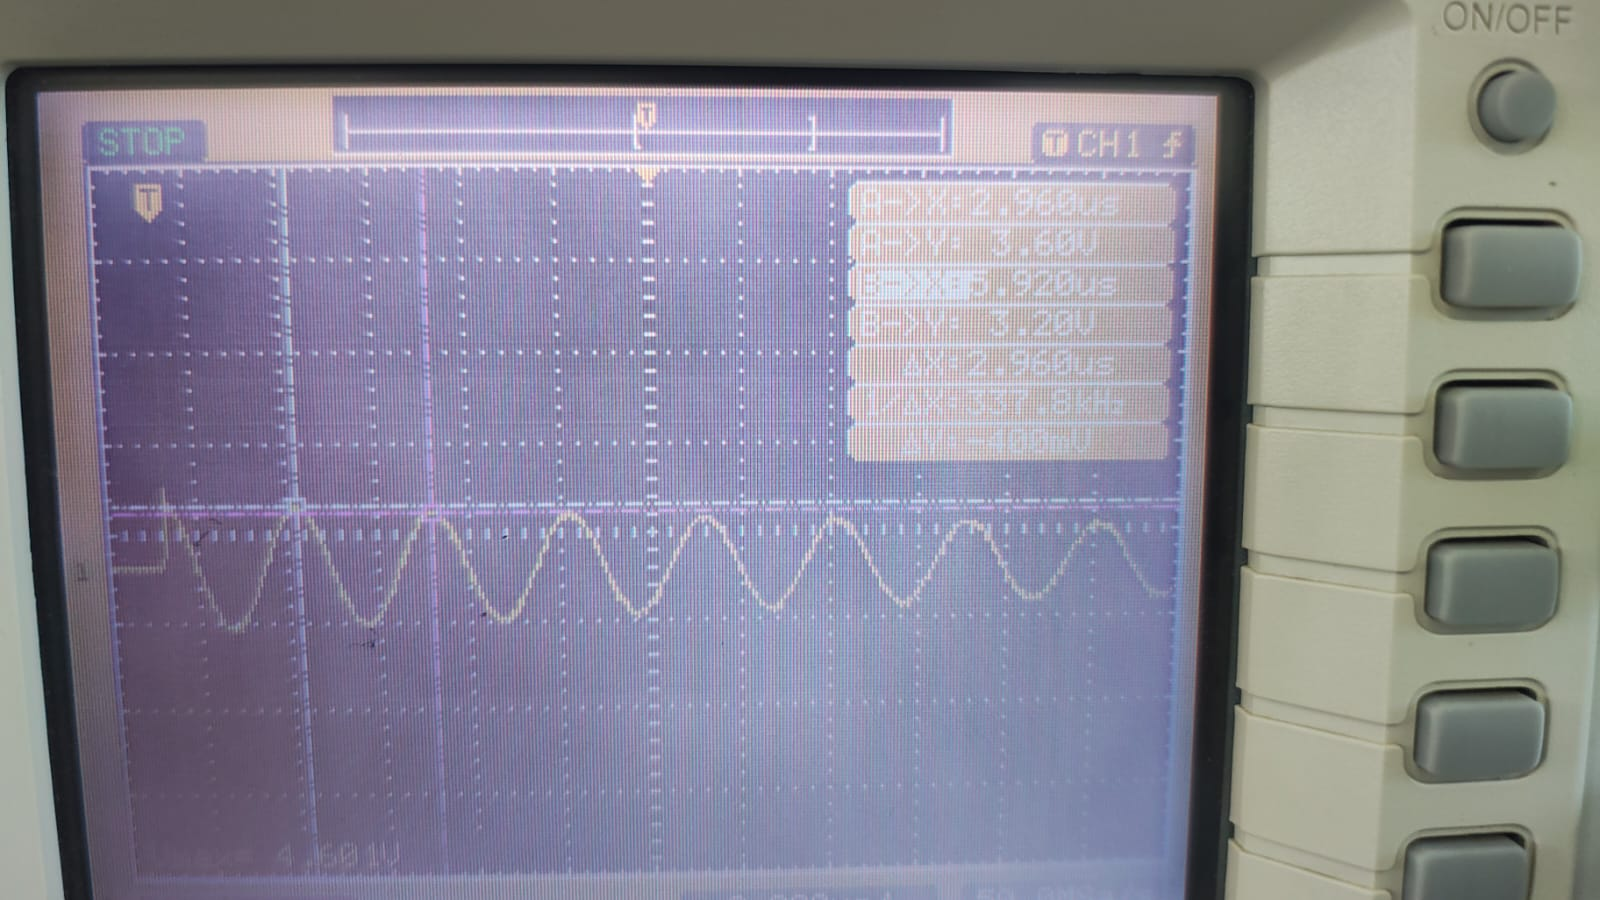
\includegraphics[width=0.5\columnwidth]{fig1.jpeg}}
  \hspace{\fill}
  {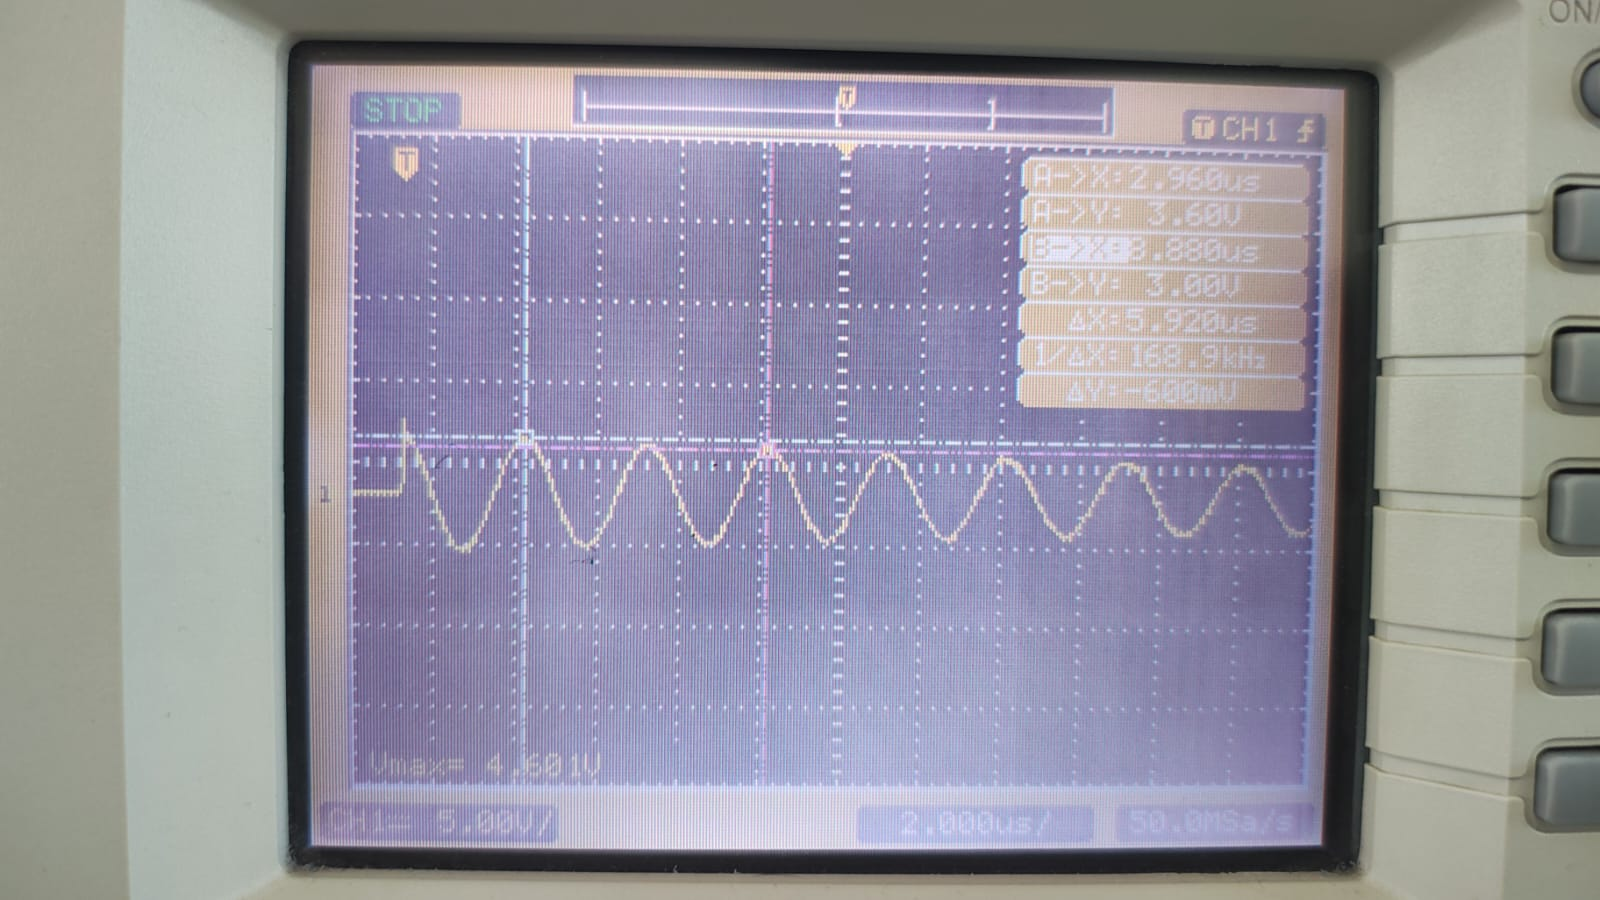
\includegraphics[width=0.5\columnwidth]{fig2.jpeg}}
  \caption{Response}
\end{figure}

\begin{figure}[!htb]
  {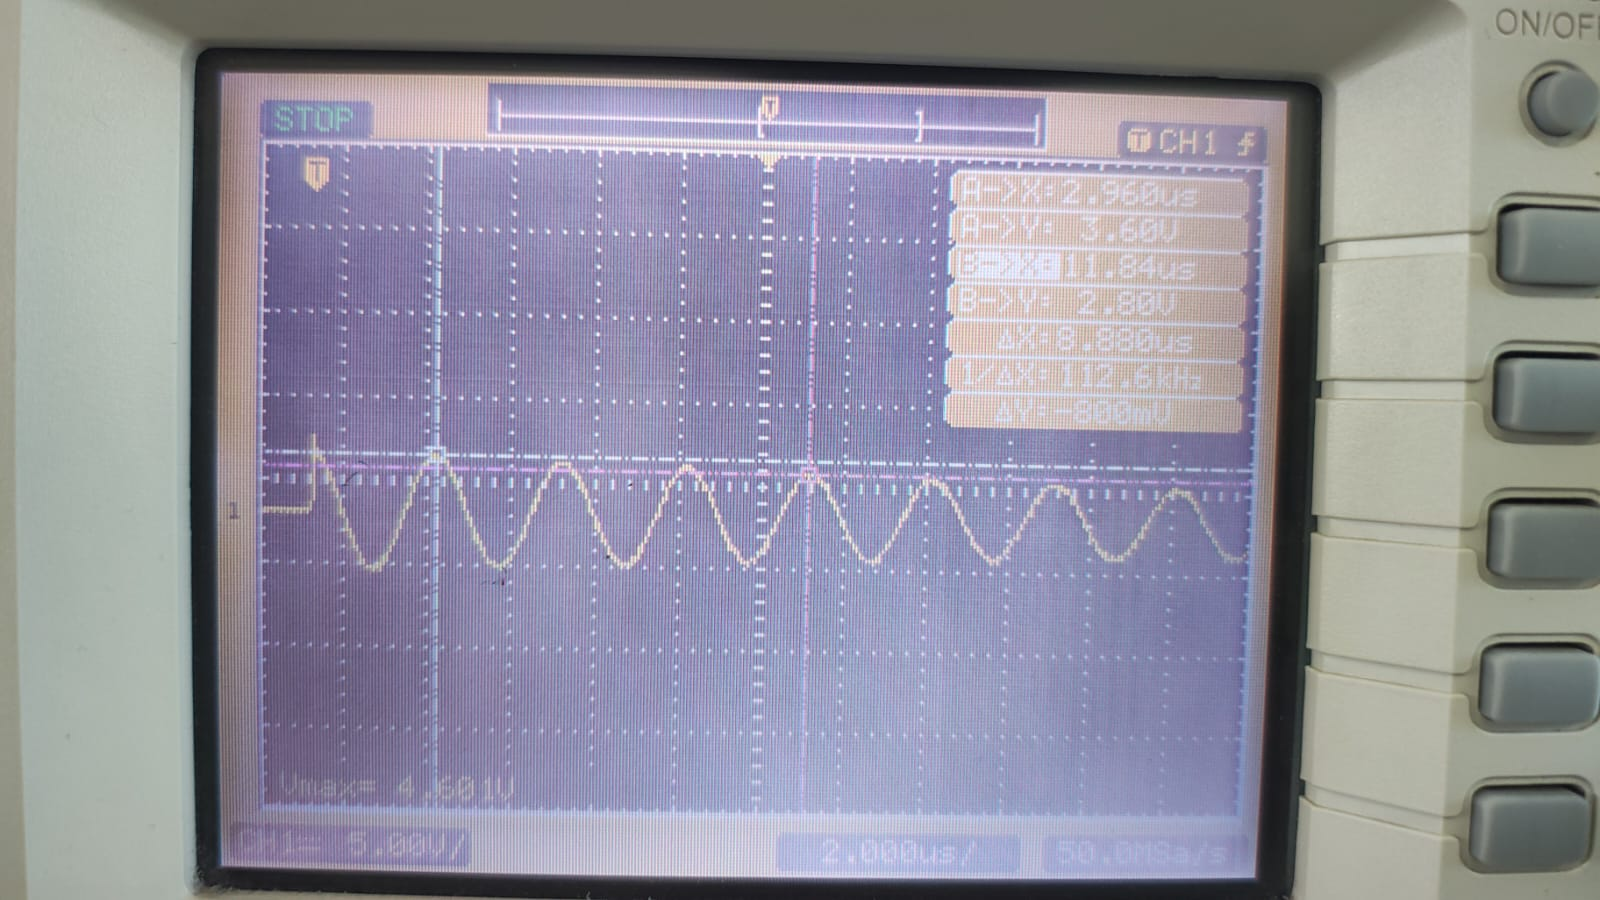
\includegraphics[width=0.5\columnwidth]{fig3.jpeg}}
  \hspace{\fill}
  {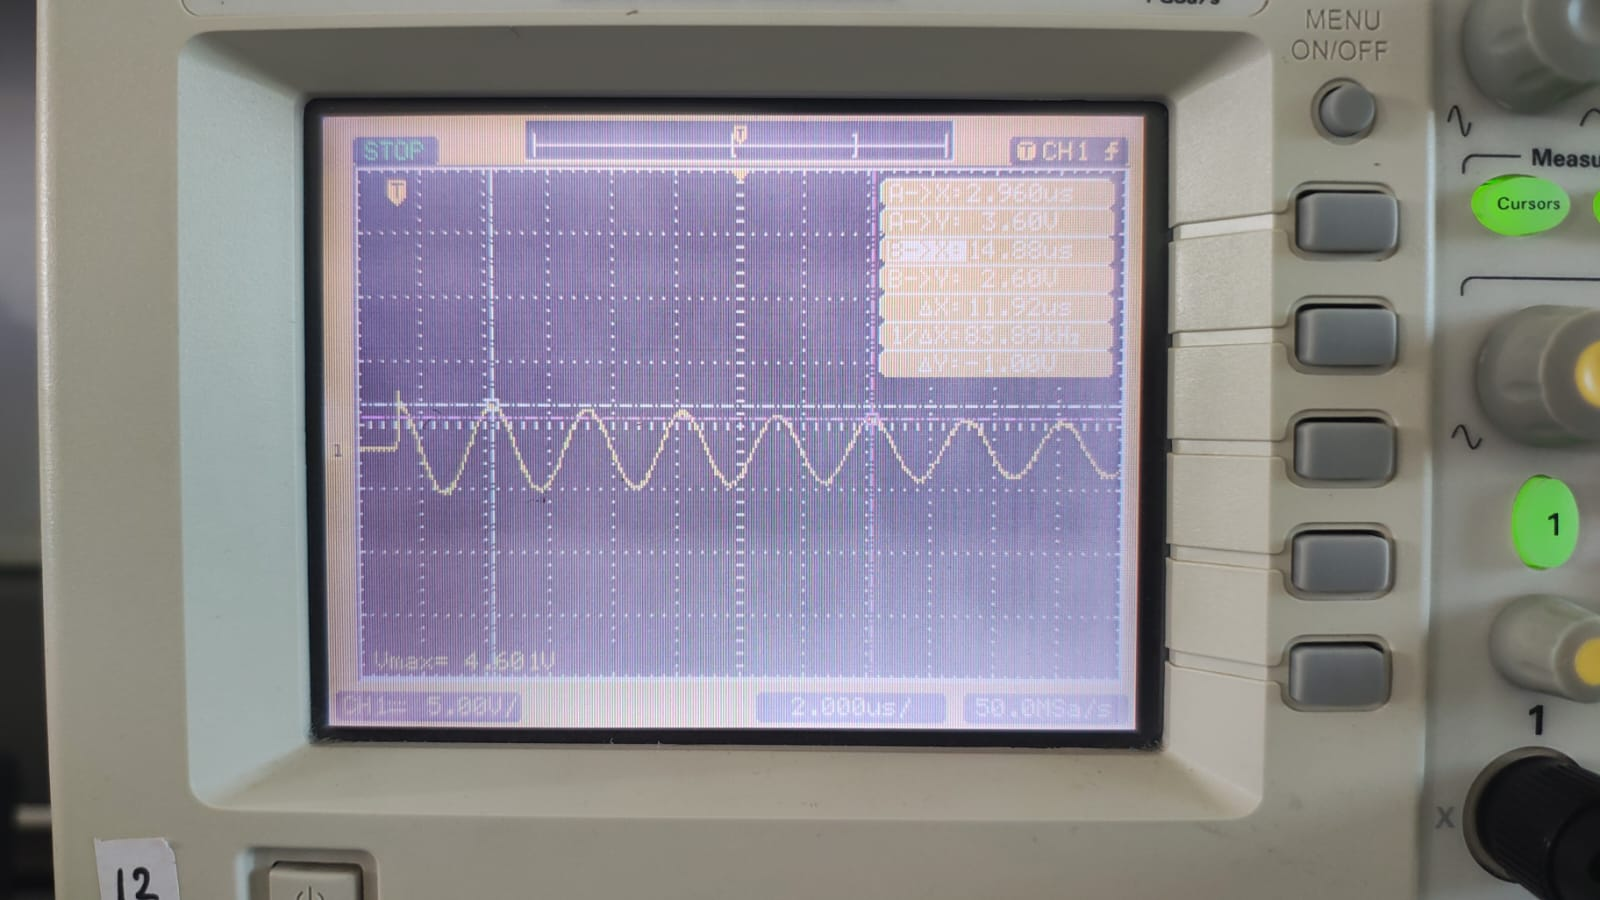
\includegraphics[width=0.5\columnwidth]{fig4.jpeg}}
  \caption{Response}
\end{figure}

\begin{figure}[!htb]
  {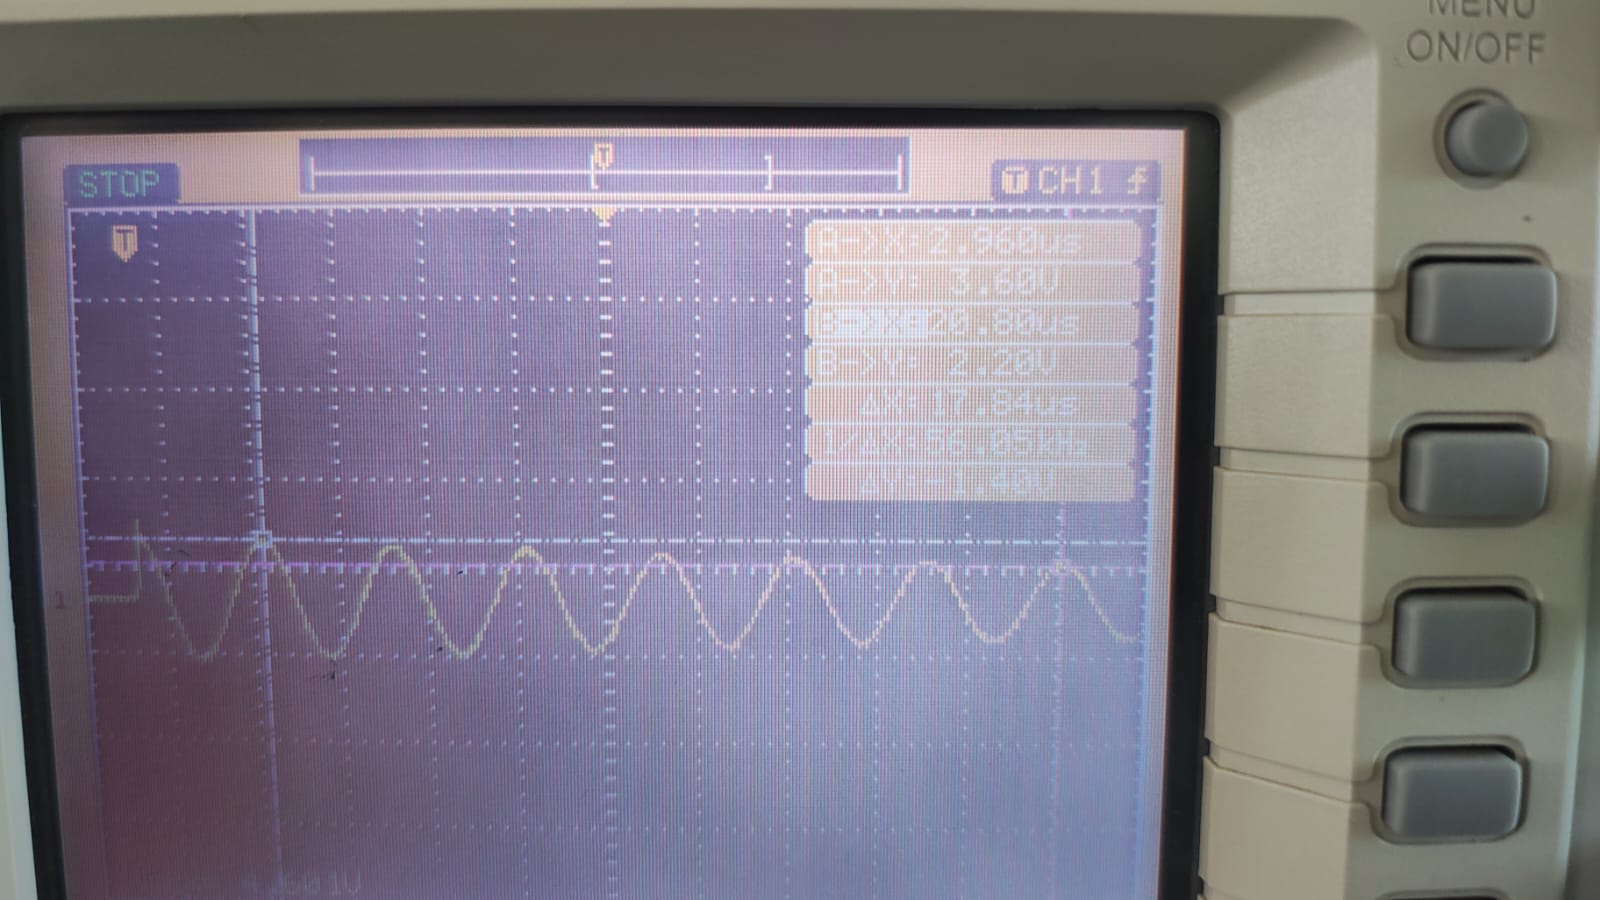
\includegraphics[width=0.5\columnwidth]{fig5.jpeg}}
  \hspace{\fill}
  \caption{Response}
\end{figure}
\end{document}
